% Created 2016-08-17 Wed 14:38
\documentclass[tikz]{standalone}

\usepackage[utf8]{inputenc}
\usepackage[T1]{fontenc}
\usepackage{helvet}
\usepackage{../../templates/msc}

\renewcommand{\familydefault}{\sfdefault}

\tikzset{
every picture/.style={
line width=1pt
}}

\usepackage{tikz}
\author{Holger Karl}
\date{\today}
\title{}


\begin{document}
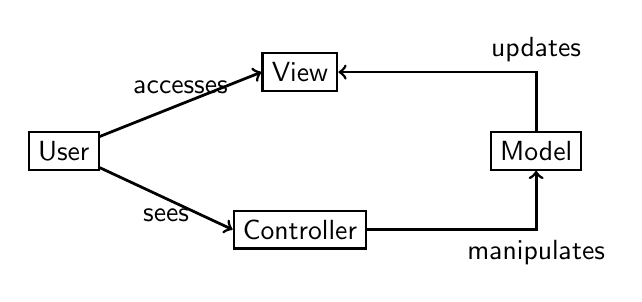
\begin{tikzpicture}[auto, xscale=3,
block/.style = {rectangle, draw=black, thick, align=left}]
\node[block] at (0,1) (u) {User};
\node[block] at (1,0) (c) {Controller};
\node[block] at (1,2) (v) {View};
\node[block] at (2,1) (m) {Model};

\draw[->] (c) -| node[below] {manipulates} (m); 
\draw[->] (m) |- node[above] {updates} (v); 
\draw[->] (u) -- node[above] {accesses} (v.west); 
\draw[->] (u) -- node[below] {sees} (c.west); 

  % \node [block]  at (0,1) (sender) {\textbf{Sender:} \\x = native data;\\px = pack(x);
  %   \\send(px);};
  % \node [block] at (2,3) (idl) {Data definition file};
  % \node [block] at (2,2) (idlcomp) {IDL compiler};
  % \node [block] at (1,1) (pack) {pack()}; 
  % \node [block] at (3,1) (unpack) {unpack()}; 
  % \node [block]  at (4,1) (receiver) {\textbf{Receiver:} \\px =  receive();\\x = unpack(px);
  %   \\//use native data in x };
  % %
  % \draw [->] (idl) -- (idlcomp); 
  % \draw [->] (idlcomp) -- (pack); 
  % \draw [->] (idlcomp) -- (unpack); 
  % \draw (-1,-1) -- (5,-1);
  % \draw [->] (sender) -- (0, -1); 
  % \draw [->] (4, -1) -- (receiver); 
  % \draw  [->] (sender.east) to [bend left=80] (pack.west) ; 
  % \draw  [->] (pack.west) to [bend left=45] (sender.east) ; 
  % \draw  [->] (receiver.west) to [bend left=45] (unpack.east) ; 
  % \draw  [->] (unpack.east) to [bend left=45] (receiver.west) ; 
  % \path (sender) edge [bend north ] node [right] {} (pack);
\end{tikzpicture}
\end{document}